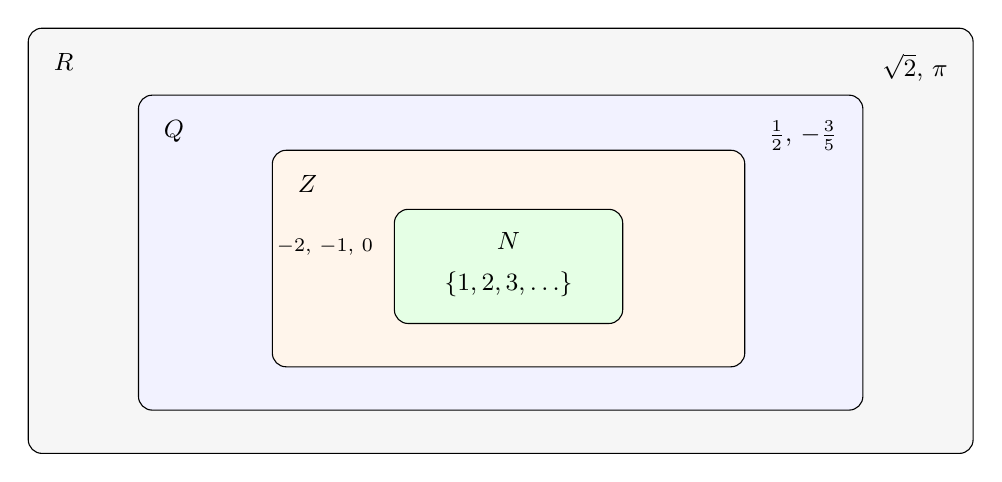
\begin{tikzpicture}[font=\small]
  \draw[rounded corners=5pt,fill=gray!7] (0,0) rectangle (12,5.4);
  \node[anchor=north west] at (0.2,5.2) {$\mathbb{R}$};
  \node[anchor=north east] at (11.8,5.2) {$\sqrt{2},\,\pi$};
  \draw[rounded corners=5pt,fill=blue!5] (1.4,0.55) rectangle (10.6,4.55);
  \node[anchor=north west] at (1.6,4.35) {$\mathbb{Q}$};
  \node[anchor=north east] at (10.4,4.35) {$\frac12,\,-\frac35$};
  \draw[rounded corners=5pt,fill=orange!8] (3.1,1.1) rectangle (9.1,3.85);
  \node[anchor=north west] at (3.3,3.65) {$\mathbb{Z}$};
  \node[anchor=north east] at (4.5,2.85) {\scriptsize $-2,\,-1,\,0$};
  \draw[rounded corners=5pt,fill=green!10] (4.65,1.65) rectangle (7.55,3.1);
  \node at (6.1,2.7) {$\mathbb{N}$};
  \node at (6.1,2.15) {$\{1,2,3,\ldots\}$};
\end{tikzpicture}
